\documentclass{article}
\usepackage[margin=1in]{geometry} % For setting page margins
\usepackage{amsmath}
\usepackage{amssymb} % For math symbols and equations
\usepackage{graphicx} % For including images
\usepackage{hyperref} 
\usepackage{enumitem}
\usepackage{float}
\usepackage{listings}
\usepackage{xcolor}
\usepackage{caption}

\renewcommand{\thesection}{\arabic{section}.}
\renewcommand{\thesubsection}{(\alph{subsection})}

\lstdefinestyle{matlabstyle}{
    language=Matlab,              % Specify the language
    basicstyle=\ttfamily\footnotesize\color{black}, % Code font
    keywordstyle=\color{blue}\bfseries, % Keywords in blue
    stringstyle=\color{orange},    % Strings in green
    commentstyle=\color{magenta}, % Comments in magenta
    numbers=left,                 % Line numbers on the left
    numberstyle=\tiny\color{black},% Line number style
    stepnumber=1,                 % Line number increment
    breaklines=true,              % Line breaking
    frame=single,                 % Border around code
    backgroundcolor=\color{white},
    tabsize=4,                    % Tab size
    showstringspaces=false,       % Don't show spaces in strings
}

\begin{document}

\title{
    \begin{tabular}{@{}l@{}}
        \textbf{Class:} Robust Multivariate Control \\
        \textbf{Professor:} Dr. Sean Humbert \\
        \textbf{TAs:} Santosh Chaganti \\
        \textbf{Student:} Steve Gillet \\
        \textbf{Date:} \today \\
        \textbf{Assignment:} Homework 7
    \end{tabular}
}

\author{}
\date{}

\maketitle

\section{}
\textit{In this problem you will analyze the robustness properties of a F-16 equipped with a lateral regulator. We consider the lateral dynamics $(\beta, \phi, p, r)$ augmented with aileron and rudder actuator dynamics $\left(\delta_a, \delta_r\right)$ and a washout filter $\left(x_w\right)$ in the yaw channel. The state vector of the augmented dynamics is $\left(\beta, \phi, p, r, \delta_a, \delta_r, x_w\right)$. The outputs of the model include $\left(r_w, p, \beta, \phi\right)$ where $r_w$ is the washed out yaw rate. Assume a static controller $u = K e$ where
\[
K = \begin{bmatrix}
-0.56 & -0.44 & -0.11 & -0.35 \\
-1.19 & -0.21 & -0.44 & 0.26
\end{bmatrix}.
\]
An m-file with the augmented system $A, B, C, D$ matrices and controller gains $K$ is available for download on the course website. For the analysis, assume that the plant is subject to an unstructured inverse multiplicative output uncertainty $\bar{G} = (I - W_o \Delta)^{-1} G$ and the desired performance metric is attenuation of measurement noise $n$ at the output $y$, as described.}

\subsection{} 
\textit{Draw a block diagram of the overall system including the weighting functions described below and label $w, z, v, u, y_{\Delta}$ and $u_{\Delta}$.}

\begin{figure}[H]
    \centering
    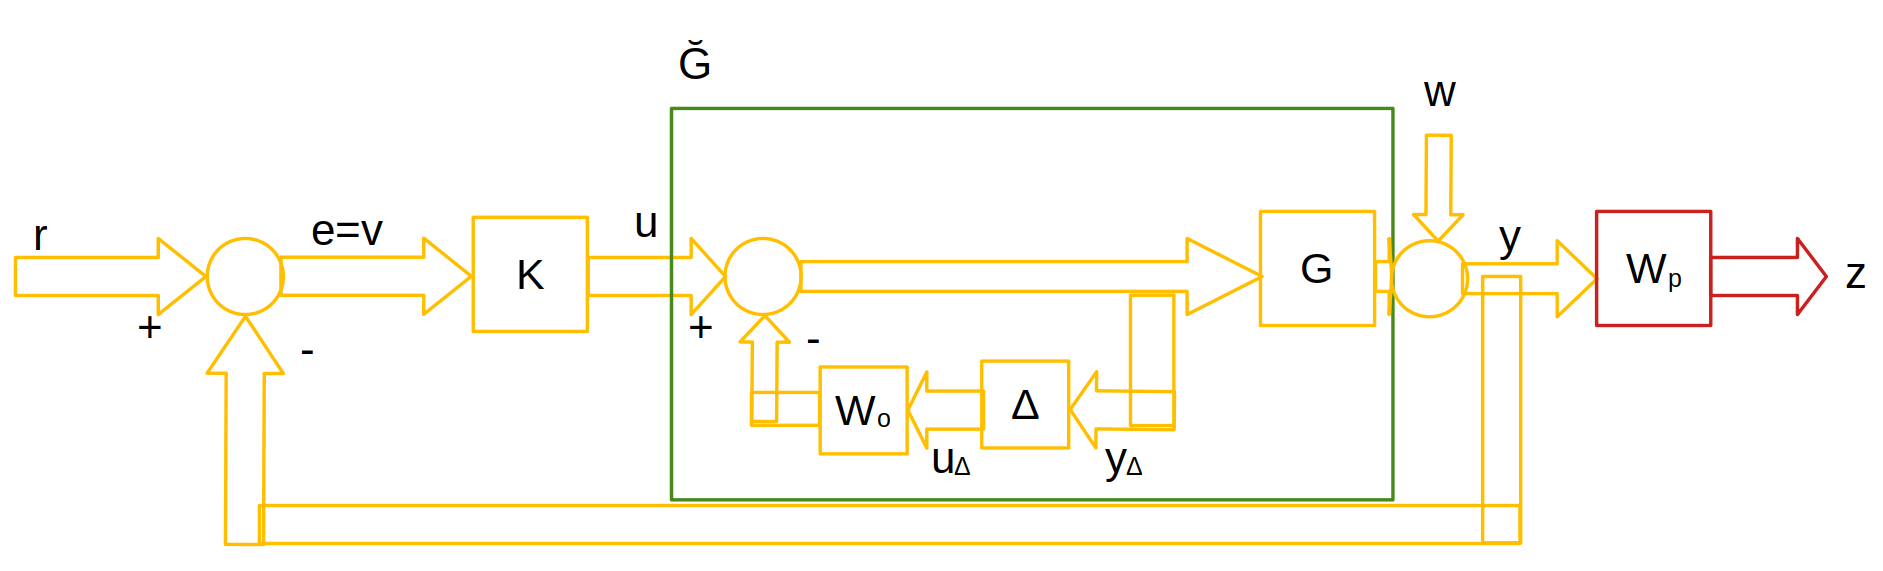
\includegraphics[width=\textwidth]{1blockDiagram.png}
    \caption{Block diagram of the overall system with labeled components.}
    \label{fig:1blockDiagram}
\end{figure}

\subsection{} 
\textit{Compute the generalized plant $P$ and close the lower LFT (with $\Delta \neq 0$) to compute $N$. What are the corresponding tests for nominal performance and robust stability?}

Writing $y_{\Delta}$, $v$, $z$ in terms of $u_{\Delta}$, $w$, $u$:

\begin{align*}
    y_{\Delta} &= u - W_o u_{\Delta} \\
    z &= W_p(w + G(u - W_o u_{\Delta})) \\
    v &= -y \\
      &= -w -G(u-W_o u_{\Delta}) \\
\end{align*}

\[
\begin{bmatrix}
    y_{\Delta} \\
    z \\
    v
\end{bmatrix}
=
\begin{bmatrix}
    -W_o & 0 & I \\
    -W_p G W_o & W_p & W_p G \\
    G W_o & -I & -G
\end{bmatrix}
\begin{bmatrix}
    u_{\Delta} \\
    w \\
    u
\end{bmatrix}
\]

Closing lower LFT:
\begin{align*}
    N = F_l(P,K) &= P_{11} + P_{12} K (I - P_{22} K)^{-1} P_{21} \\
    &= \begin{bmatrix} -W_o & 0 \\ -W_p G W_o & W_p \end{bmatrix} + \begin{bmatrix} I \\ W_p G \end{bmatrix} K (I + G K)^{-1} \begin{bmatrix} G W_o & -I \end{bmatrix} \\
    &= \begin{bmatrix} -W_o + K (I + G K)^{-1} G W_o & -K (I + G K)^{-1} \\ -W_p G W_o + W_p G K (I + G K)^{-1} G W_o & W_p - W_p G K (I + G K)^{-1} \end{bmatrix} \\
    &= \begin{bmatrix} S_I W_o & -K S_O \\ -W_p S_O G W_o & W_p T_O \end{bmatrix} \\
\end{align*}

The test for robust stability is comes from the $N_{11}$ block so $S_I W_o$.
The test for nominal performance comes from the $N_{22}$ block so $W_p T_O$.
Need those $H_\infty$ norms to be less than 1.

\subsection{} 
\textit{Assume a performance weighting function to be $W_p(s) = w_p(s) I$ where $w_p(s) = (s / M + \omega_B^*)/(s + \omega_B^* A)$, with $A = 4$; $M = 10$; $\omega_B^* = 3$. Does the system satisfy this nominal performance criterion you derived in part (b)?}

I created N in Matlab using the weighting functions and state space models including the state space model for the controller included in the hint below and the state space model for the plant provided.

\begin{lstlisting}[style=matlabstyle]
plantSS = ss(A,B,C,D);
controllerSS = ss(cA,cB,cC,cD);

Ti = controllerSS*plantSS*inv(eye(size(controllerSS*plantSS)) + controllerSS*plantSS);
To = plantSS*controllerSS*inv(eye(size(plantSS*controllerSS)) + plantSS*controllerSS);
So = inv(eye(size(plantSS*controllerSS)) + plantSS*controllerSS);
Si = inv(eye(size(controllerSS*plantSS)) + controllerSS*plantSS);

s = tf('s');
Wp = (s/10 + 3)/(s+3*4)*eye(4);
Wo = (0.02*s+0.05)/(0.02*s/0.4+1)*eye(2);

N = [Si*Wo -K*So; -Wp*So*plantSS*Wo Wp*To];    
\end{lstlisting}

I then plotted the sigma plots and computed the $H_\infty$ norm for the $N_{22}$ block.

\begin{figure}[H]
    \centering
    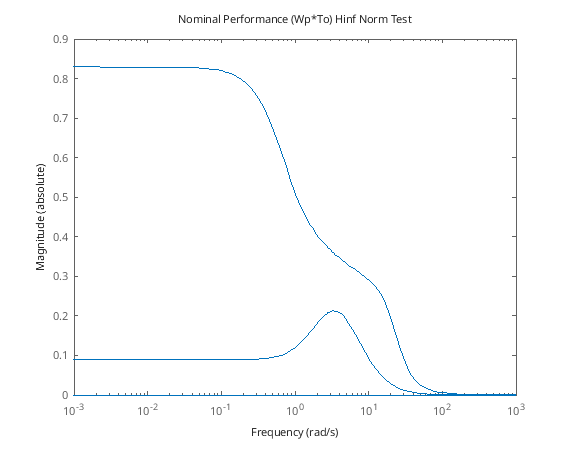
\includegraphics[width=\textwidth]{1performance.png}
    \label{fig:1performance}
\end{figure}

The $H_\infty$ norm is 0.8292 which is less than 1 so the system satisfies the nominal performance criterion.

\subsection{} 
\textit{Assume an uncertainty weighting function to be $W_o(s) = w_o(s) I$ where $w_o(s) = (\tau s + r_0)/(\tau s / r_{\infty} + 1)$, with $\tau = 0.02$, $r_0 = 0.05$, $r_{\infty} = 0.4$, and full (unstructured) uncertainty. Is the system robustly stable using the criterion you derived in part (b)?}
\textit{Hint: to compute the state space model for the controller, assume $D = K$ (static gain) and the $A, B, C$ matrices are all zeros with appropriate dimensions.}

I used the same technique to compute and plot the robust stability for the system using $W_p T_O$ from the $N_{22}$ block for robust stability.
The $H_\infty$ norm is 0.4679 which is less than 1 so the system satisfies the robust stability criterion.

\begin{figure}[H]
    \centering
    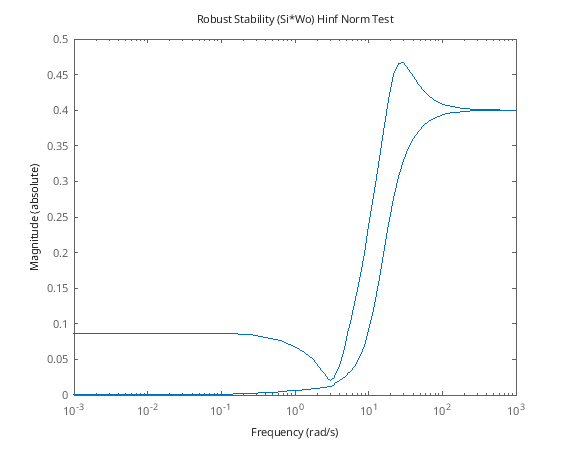
\includegraphics[width=\textwidth]{1stability.png}
    \label{fig:1stability}
\end{figure}

\section{}
\textit{Consider a model of the longitudinal dynamics of a missile
\[
\begin{aligned}
\frac{d}{d t} \begin{bmatrix} \alpha \\ q \end{bmatrix} &= \begin{bmatrix} Z_\alpha & Z_q \\ M_\alpha & 0 \end{bmatrix} \begin{bmatrix} \alpha \\ q \end{bmatrix} + \begin{bmatrix} Z_{\delta_u} \\ M_{\delta_u} \end{bmatrix} \delta_u \\
n_z &= \begin{bmatrix} Z_\alpha & 0 \end{bmatrix} \begin{bmatrix} \alpha \\ q \end{bmatrix} + Z_{\delta_u} \delta_u
\end{aligned}
\]
where the states are the angle of attack $\alpha$, the pitch rate $q$, $n_z$ is the output (normal acceleration), $\delta_u$ is the tail deflection input. Assume the following variations in stability derivatives: $M_\alpha = M_\alpha^0 + \delta_\alpha$ and $Z_q = Z_q^0 + \delta_q$. Generate the analytical state space model as discussed in lecture for the extended plant $N$ by "pulling out the deltas" for this case of structured uncertainty. Assume $w = \delta_u$, $z = n_z$ and $\Delta = \operatorname{diag}\{\delta_\alpha, \delta_q\}$.}

I started with the state space block diagram from the input to the output showing how the different states, dynamics, and uncertainties are related.

\begin{figure}[H]
    \centering
    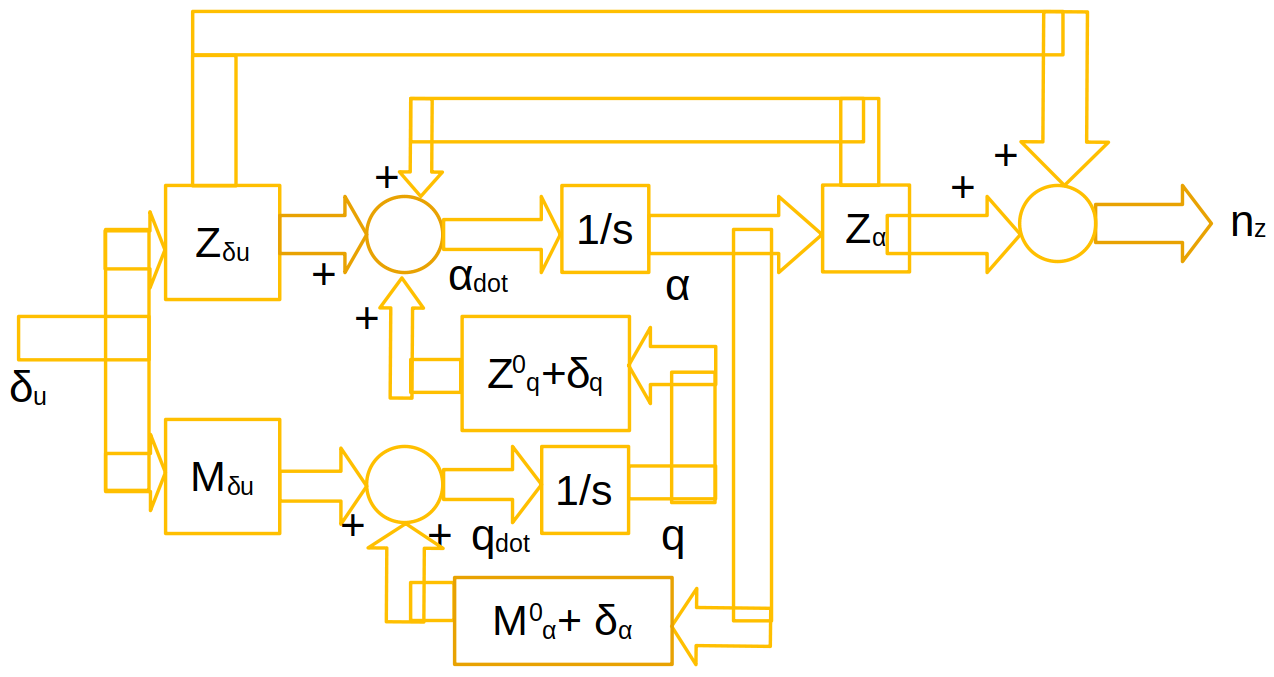
\includegraphics[width=\textwidth]{2blockDiagram.png}
    \label{fig:2blockDiagram}
    \caption{State Space Block Diagram of Longitudinal Missile Dynamics}
\end{figure}

Then I "pulled out the deltas" so that those uncertainties can be treated as inputs and outputs.

\begin{figure}[H]
    \centering
    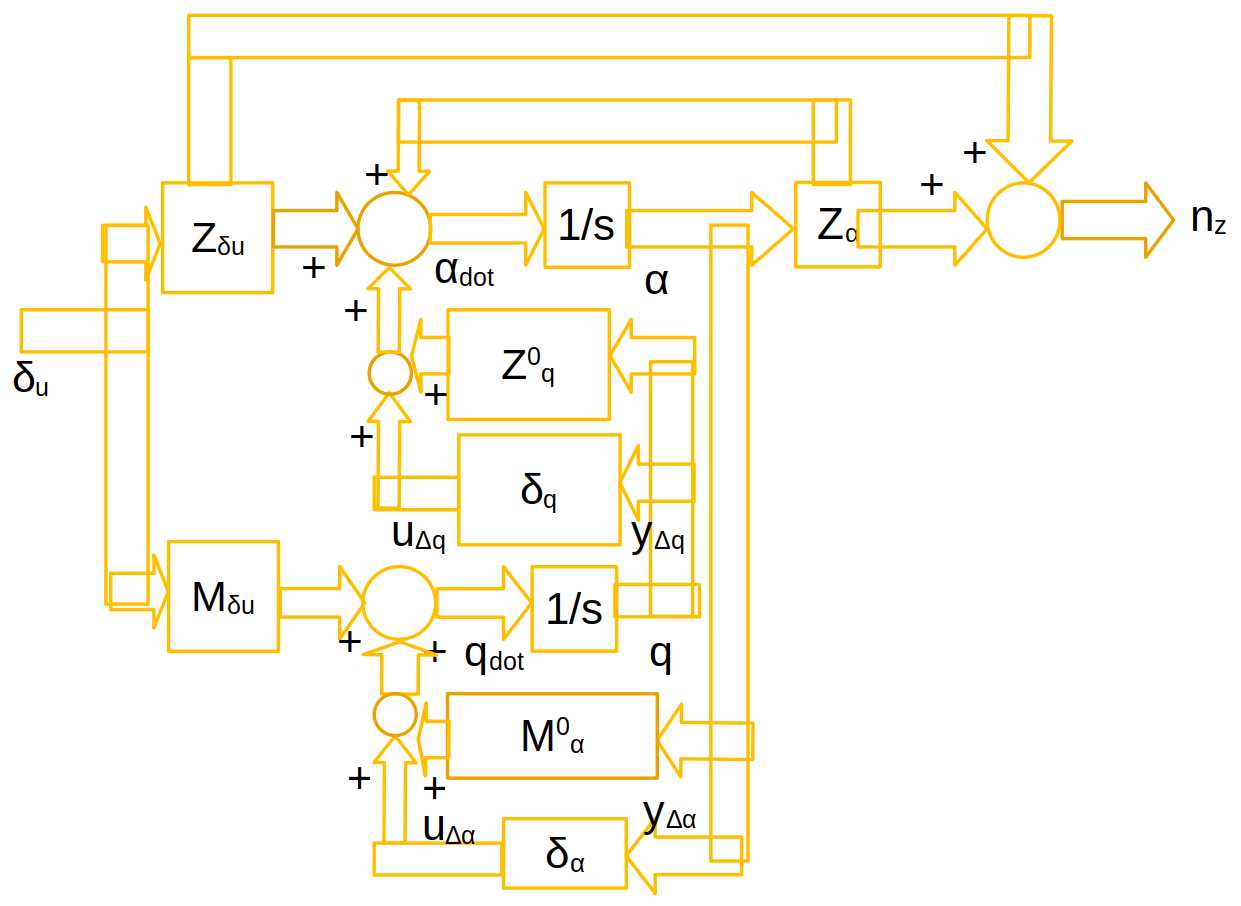
\includegraphics[width=\textwidth]{2blockDeltaPulled.png}
    \label{fig:2blockDeltaPulled}
    \caption{Block Diagram with Deltas Pulled Out}
\end{figure}

Then I wrote out the state space equations based on what I had done in the block diagrams, starting with including the $u_\Delta$s and $y_\Delta$s as separate inputs and outputs and then stacking them together to get the full anaylitcal state space quation in (d) and (e).

\begin{align*}
&\text{(a)} \quad
\begin{bmatrix}
\dot{\alpha} \\
\dot{q}
\end{bmatrix}
=
\begin{bmatrix}
Z_\alpha & Z^0_q \\
M^0_\alpha & 0
\end{bmatrix}
\begin{bmatrix}
\alpha \\
q
\end{bmatrix}
+
\begin{bmatrix}
u_{\Delta_q} \\
u_{\Delta_\alpha}
\end{bmatrix}
+
\begin{bmatrix}
Z_{\delta_u} \\
M_{\delta_u} 
\end{bmatrix}
\delta_u \\
&\text{(b)} \quad
y_{\Delta_q} = q, \quad y_{\Delta_\alpha} = \alpha \\
&\text{(c)} \quad
n_z =
\begin{bmatrix}
Z_\alpha & 0
\end{bmatrix}
\begin{bmatrix}
\alpha \\
q
\end{bmatrix}
+ Z_{\delta_u} \delta_u \\
&\text{(d)} \quad
\begin{bmatrix}
\dot{\alpha} \\
\dot{q}
\end{bmatrix}
=
\begin{bmatrix}
Z_\alpha & Z_q^0 \\
M^0_\alpha & 0
\end{bmatrix}
\begin{bmatrix}
\alpha \\
q
\end{bmatrix}
+
\begin{bmatrix}
1 & 0 & Z_{\delta_u} \\
0 & 1 & M_{\delta_u}
\end{bmatrix}
\begin{bmatrix}
u_{\Delta_q} \\
u_{\Delta_\alpha} \\
\delta_u
\end{bmatrix} \\
&\text{(e)} \quad
\begin{bmatrix}
Y_{\Delta_\alpha} \\
Y_{\Delta_q} \\
n_z
\end{bmatrix}
=
\begin{bmatrix}
1 & 0 \\
0 & 1 \\
Z_\alpha & 0
\end{bmatrix}
\begin{bmatrix}
\alpha \\
q
\end{bmatrix}
+
\begin{bmatrix}
0 & 0 & 0 \\
0 & 0 & 0 \\
0 & 0 & Z_\delta
\end{bmatrix}
\begin{bmatrix}
u_{\Delta_q} \\
u_{\Delta_\alpha} \\
\delta_u
\end{bmatrix} \\
&\text{(f)} \quad
N = (s I - A)^{-1} B \\
&\quad =
\begin{bmatrix}
1 & 0 \\
0 & 1 \\
Z\alpha & 0
\end{bmatrix}
(s I -
\begin{bmatrix}
Z\alpha & Z_q^0 \\
M_\alpha^0 & 0
\end{bmatrix})^{-1}
\begin{bmatrix}
1 & 0 & Z_{\delta_u} \\
0 & 1 & M_{\delta_u}
\end{bmatrix} \\
&\quad =
\begin{bmatrix}
1 & 0 \\
0 & 1 \\
Z_\alpha & 0
\end{bmatrix}
\begin{bmatrix}
s - Z_\alpha & s - Z_q^0 \\
s-M_\alpha^0 & s
\end{bmatrix}^{-1}
\begin{bmatrix}
1 & 0 & Z_{\delta_u} \\
0 & 1 & M_{\delta_u}
\end{bmatrix}
\end{align*}

Then you can see where I wrote out what that Transfer Function would look like from the input to the output with the uncertainties.

\section{}

\textit{Consider the following lateral flight dynamics model for the A-4D aircraft:}

\[
\frac{d}{d t}
\begin{bmatrix}
\beta \\
r
\end{bmatrix}
=
\begin{bmatrix}
Y_\beta / u_0 & -\left(1 - Y_r / u_0\right) \\
N_\beta & N_r
\end{bmatrix}
\begin{bmatrix}
\beta \\
r
\end{bmatrix}
+
\begin{bmatrix}
0 & Y_{\delta_r} / u_0 \\
N_{\delta_a} & N_{\delta_r}
\end{bmatrix}
\begin{bmatrix}
\delta_a \\
\delta_r
\end{bmatrix}.
\]

\textit{Assume the sea level reference flight condition (Condition 1) from the attached data sheet, and Mach 1 at sea level is $1126 \, \text{ft/s}$ (use this to compute $u_0$). Build the state space $A$ and $B$ matrices using the regular stability and control derivatives $\left(Y_\beta, N_\beta, N_r, Y_{\delta_r}, N_{\delta_a}, N_{\delta_r}\right)$, not the 'primed' derivatives, and assume $Y_r = 0$. Also assume the $C$ matrix is the identity so that the outputs are the two states $\beta$ and $r$.}

\subsection{}

\textit{Using the nominal plant, synthesize a $H_{\infty}$ controller using hinfsyn with a disturbance rejection performance weighting function $W_p(s) = w_p(s) I$ where $w_p(s) = \left(s / M + \omega_B^*\right) / \left(s + \omega_B^* A\right)$, with $A = 0.005$; $M = 2$; $\omega_B^* = 1$. Does the closed loop system satisfy nominal performance? Verify with a plot of $\partial[S(j \omega)]$ and $1 / \left| w_p(j \omega) \right|$.}

\subsection{}

\textit{Now allow the parameter $Y_\beta$ to have $20\%$ real uncertainty and compute $\mu\left(N_{11}\right)$. Use the MATLAB command mussv and generate the $N$ and $\Delta$ blocks using the commands $1 \mathrm{ft}$ and lftdata as was done in lecture. Does the controller you designed provide robust stability for the perturbation in $Y_\beta$?}

\subsection{}

\textit{Now compute the robust performance test $\mu(N)$ using the appropriate unstructured $\Delta_p$ and structured $\Delta$ blocks as was discussed in lecture. Does the controller you designed provide robust performance for the perturbation in $Y_\beta$?}

\subsection{}

\textit{Now add an additional perturbation of $30\%$ real uncertainty of the parameter $N_\beta$ and check to see if your controller provides robust stability and robust performance for this uncertainty case.}

\end{document}